\documentclass[12pt]{article}

\usepackage[a4paper,width=150mm,top=25mm,bottom=25mm]{geometry}

\usepackage{graphicx,url}

\usepackage[brazil]{babel}   
\usepackage[utf8]{inputenc}  
% UTF-8 encoding is recommended by ShareLaTex

\usepackage[backend=biber]{biblatex}
\addbibresource{relatorio.bib}

\usepackage[activate={true,nocompatibility},final,tracking=true,kerning=true,spacing=true,factor=1100,stretch=10,shrink=10]{microtype}
% activate={true,nocompatibility} - activate protrusion and expansion
% final - enable microtype; use "draft" to disable
% tracking=true, kerning=true, spacing=true - activate these techniques
% factor=1100 - add 10% to the protrusion amount (default is 1000)
% stretch=10, shrink=10 - reduce stretchability/shrinkability (default is 20/20)

\usepackage{float}
\usepackage{listings}

\usepackage{caption}

\usepackage{color}
 
\definecolor{codegreen}{rgb}{0,0.6,0}
\definecolor{codegray}{rgb}{0.5,0.5,0.5}
\definecolor{codepurple}{rgb}{0.58,0,0.82}
\definecolor{backcolour}{rgb}{0.95,0.95,0.92}
 
\lstdefinestyle{mystyle}{
    backgroundcolor=\color{backcolour},   
    commentstyle=\color{codegreen},
    keywordstyle=\color{magenta},
    numberstyle=\tiny\color{codegray},
    stringstyle=\color{codepurple},
    basicstyle=\footnotesize,
    breakatwhitespace=false,         
    breaklines=true,                 
    captionpos=b,                    
    keepspaces=true,                 
    numbers=left,                    
    numbersep=5pt,                  
    showspaces=false,                
    showstringspaces=false,
    showtabs=false,                  
    tabsize=2
}
 
\lstset{style=mystyle}
     
\sloppy

\title{Análise de Métodos para Processamento de Imagens}

\author{Pedro Pillon Vanzella}

\begin{document} 

\maketitle
     
\section{Introdução}\label{sec:introducao}

Dentre as muitas aplicações dos métodos numéricos, uma das mais populares é o processamento de imagens~\cite{acharya:2005}. Estes métodos são empregados em um número de meios, como fotografia digital, tratamento de imagens, produção de vídeo e jogos.

Os problemas de redimensionamento e rotação de imagens são alguns dos mais simples e ao mesmo tempo mais comuns. Analisemos o problema de um jogo: imagens são utilizadas como texturas em praticamente todos os polígonos e um jogo. É possível que elas devam ser redimensionadas ou rotacionadas a cada quadro, e potencialmente milhares delas serão exibidas ao mesmo tempo. É interessante, então, que se faça uso de algoritmos de custo computacional mais baixo possível, de modo a tornar a experiência do jogo mais fluida e agradável.

Para este fim, utilizaremos o ambiente GNU Octave, que é um software livre para a computação numérica e científica~\cite{eaton:2008}.

Para os métodos de redimensionamento analisaremos as interpolações \textit{Nearest Neighbor} (Seção~\ref{sec:redimensionamento:nearest}), Bicúbica (Seção~\ref{sec:redimensionamento:bicubica}) e Bilinear (Seção~\ref{sec:redimensionamento:bilinear}). Para os métodos de rotação, analisaremos os métodos de Rotação por \textit{Nearest Neighbor} (Seção~\ref{sec:rotacao:nearest}), por Interpolação Bilinear (Seção~\ref{sec:rotacao:bilinear}) e por Interpolação Bicúbica (Seção~\ref{sec:rotacao:bicubica}).

Utilizaremos sempre a mesma imagem como base, de modo a podermos comparar os resultados. Podemos vê-la na Figura~\ref{fig:vaca:semnada}.

Será feita uma comparação do tempo de execução de cada algoritmo, bem como da qualidade da imagem gerada, de modo a tomar uma decisão quanto à melhor técnica para o caso hipotético de texturas em um jogo 3D.

\begin{figure}[H]
\centering
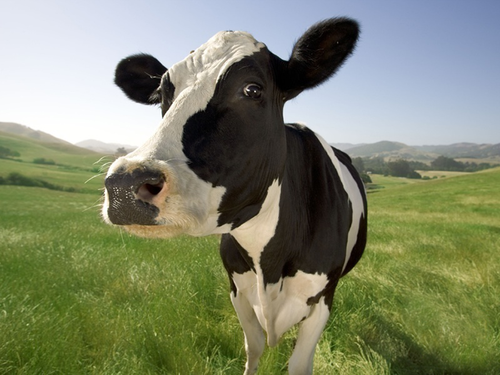
\includegraphics[width=0.5\textwidth]{cow_small.png}
\caption{Uma simpática vaquinha}
\label{fig:vaca:semnada}
\end{figure}

\section{Redimensionamento de Imagens}\label{sec:redimensionamento}

Redimensionamento de imagens é um processo não trivial, que envolve um balanço entre eficiência e qualidade de resultado~\cite{kopf:2011}.

Dentre os vários algoritmos existentes para esta tarefa, vamos abordar os três mais comuns~\cite{han2013}: Interpolação por \textit{Nearest Neighbor}, Interpolação Bilinear e Interpolação Bicúbica.

É importante analisarmos exatamente este balanço de qualidade e performance. Uma solução que gere resultados perfeitos, mas demore muito não seria útil, pois deve ser executada milhares de vezes a cada quadro, e isto reduziria a performance do jogo. De mesmo modo, uma solução mais rápida não é útil caso gere resultados muito ruins, ou introduza artefatos que causem discontinuidades nas texturas, pois isso quebraria a ilusão de 3D no jogo.

Desta forma, a escolha de melhor método é, possivelmente, uma combinação de avaliações objetivas e subjetivas. Descarta-se as soluções que geram resultados pouco visualmente agradáveis\footnote{uma avaliação completamente subjetiva}, e elege-se como melhor o que, dentre os que sobraram, traz resultados mais rápidos\footnote{uma avaliação objetiva}.

\subsection{Interpolação por \textit{Nearest Neighbor}}\label{sec:redimensionamento:nearest}
Interpolação por \textit{Nearest Neighbor} é o método mais simples de se implementar, bem como o mais rápido~\cite{han2013}.

A idéia do algoritmo de \textit{Nearest Neighbor} é simples - simplesmente copiar os pixels mais próximos para o lugar dos que estão sendo adicionados ao se ampliar a imagem. Isto gera resultados rápidos, porém de baixa qualidade, como podemos ver na Figura~\ref{fig:vaca:nearest}.c. Há um claro serrilhado que é introduzido ao se ampliar a imagem.

Reduzir uma imagem com este algoritmo também gera resultados pouco satisfatórios: novamente serrilhado é introduzido e detalhes são perdidos. Podemos ver isto na Figura~\ref{fig:vaca:nearest}.a.

% http://tech-algorithm.com/articles/nearest-neighbor-image-scaling/

\begin{figure}[H]
    \begin{minipage}{.2\textwidth}
        \centering
        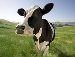
\includegraphics{cow_nearest_smallest}
        (a) 50\%
    \end{minipage}%
    \begin{minipage}{0.35\textwidth}
        \centering
        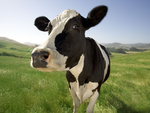
\includegraphics{cow_very_small}
        (b) Original
    \end{minipage}~
    \begin{minipage}{0.35\textwidth}
        \centering
        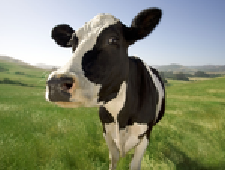
\includegraphics{cow_nearest}
        (c) 150\%
    \end{minipage}
    \caption{Redução e Ampliação com algoritmo de \textit{Nearest Neighbor}}
    \label{fig:vaca:nearest}
\end{figure}

A Tabela~\ref{tab:nearest} mostra o tempo de execução para redução e ampliação em 50\% da imagem da Figura~\ref{fig:vaca:nearest}.b. Estes dados não nos dizem muito por enquanto, mas serão úteis quando compararmos aos resultados das Seções~\ref{sec:redimensionamento:bilinear} e~\ref{sec:redimensionamento:bicubica}. Podemos apenas ver que reduzir uma imagem demora menos que ampliar a mesma. Isto se dá pelo fato de haver menos pixels a serem calculados na imagem reduzida, e é esperado.

\begin{table}[H]
    \caption{Tempo de execução}
    \centering
    \label{tab:nearest}
    \begin{tabular}{c||c}
     Redução & Ampliação \\
     \hline
     0.17s & 0.21s
    \end{tabular}
\end{table}

O código em Octave que faz esta interpolação pode ser visto na Figura~\ref{lst:scale:nearest}.

\begin{figure}[H]
\lstinputlisting[language=Octave, lastline=6]{scale-nearest.m}
\caption{Código-Fonte para interpolação \textit{Nearest Neighbor} no Octave}
\label{lst:scale:nearest}
\end{figure}

O importante na listagem da Figura~\ref{lst:scale:nearest} é a linha 5, onde uma chamada para \textsf{imresize()} é feita. Esta função encapsula a chamada para a função \textsf{interp2()}, apenas adicionando algumas garantias de que o primeiro parâmetro é uma imagem válida e verificando se há múltiplos canais\footnote{\textit{i.e.} a imagem está em RGB} e, se houver, executando a interpolação para cada um dos canais individualmente.

A função \textsf{interp2()}, por sua vez, recebe um parâmetro (passado pela \textsf{imresize()}) que diz qual tipo de interpolação deve ser feita. Neste caso, escolheu-se \emph{nearest}.

O segundo parâmetro da função \textsf{imresize()} é o fator de escala. Um fator menor que $1$ resultará em uma imagem reduzida. De mesmo modo, um valor superior a $1$ resultará em uma ampliação da imagem original.

\subsection{Interpolação Bilinear}\label{sec:redimensionamento:bilinear}

A idéia da Interpolação Bilinear é executar uma interpolação linear em uma direção e, em seguida, uma interpolação linear na outra direção.

Conforme~\cite{han2013}, podemos calcular a interpolação da seguinte maneira:

Considere quatro pontos, $A$, $B$, $C$ e $D$. Suas coordenadas são, respectivamente, $(i, j)$, $(i, j+1)$, $(i+1, j)$, $(i+1, j+1)$. Para calcular o ponto $P(u, v)$, primeiro vamos calcular um ponto $E$, que é a interpolação linear de $A$ e $B$.

\[
f(i, j+v) = [f(i, j+1) - f(i,j)]v + f(i, j)
\]

Agora vamos calcular um ponto $F$, que é a interpolação linear de $C$ e $D$.

\[
f(i + 1, j + v) = [f(i + 1, j + 1) - f(i + 1, j)]v + f(i + 1, j)
\]

Finalmente, basta calcular a interpolação linear de $E$ e $F$ para obter $P$.

\[
f(i + u, j + v) = (1-u)(1-v)f(i,j)-(1-u)vf(i, j+ 1) + u(1-v)f(i+1,j) + uvf(i + 1, j+1)
\]

Isto deve ser feito, no caso de uma imagem colorida, para cada canal da imagem.

Podemos ver na Figura~\ref{fig:vaca:bilinear} os resultados de uma redução em $50\%$ (Figura~\ref{fig:vaca:bilinear}.a) e uma ampliação em $50\%$ (Figura~\ref{fig:vaca:bilinear}.c).

A imagem ampliada apresenta um serrilhado em todas as bordas, e a definição da grama é claramente perdida.

O maior problema se encontra na imagem reduzida: uma borda preta foi gerada na imagem, devido ao processo de interpolação. Isto torna este método inútil para a redução de texturas em um jogo.

\begin{figure}[H]
    \begin{minipage}{.2\textwidth}
        \centering
        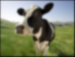
\includegraphics{cow_bilinear_smallest}
        (a) 50\%
    \end{minipage}%
    \begin{minipage}{0.35\textwidth}
        \centering
        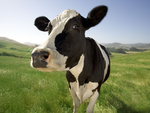
\includegraphics{cow_very_small}
        (b) Original
    \end{minipage}~
    \begin{minipage}{0.35\textwidth}
        \centering
        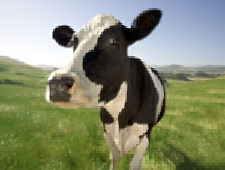
\includegraphics{cow_bilinear}
        (c) 150\%
    \end{minipage}
    \caption{Redução e Ampliação com algoritmo de Interpolação Bilinear}
    \label{fig:vaca:bilinear}
\end{figure}

Na Tabela~\ref{tab:bilinear} vemos o tempo de execução para a redução e a ampliação utilizando interpolação bilinear. Novamente, a redução é mais rápida que a ampliação, por haver menos pixels a serem calculados.

O tempo de execução da redução consta na Tabela~\ref{tab:bilinear} somente para referência, já que o resultado da mesma não é útil para o problema proposto.

\begin{table}[H]
    \caption{Tempo de execução}
    \centering
    \label{tab:bilinear}
    \begin{tabular}{c||c}
     Redução & Ampliação \\
     \hline
     0.15s & 0.23s
    \end{tabular}
\end{table}

Vemos na listagem da Figura~\ref{lst:scale:linear} o código para fazer uma interpolação bilinear em uma imagem com o Octave.

\begin{figure}[H]
\lstinputlisting[language=Octave, lastline=6]{scale-bilinear.m}
\caption{Código-Fonte para interpolação bilinear no Octave}
\label{lst:scale:linear}
\end{figure}

O código é praticamente igual ao da Figura~\ref{lst:scale:nearest}, mudando apenas a o parâmetro do método de interpolação.

A função \textsf{imresize()} novamente chamará a função \textsf{interp2()}, passando desta vez o parâmetro \emph{linear}.


\subsection{Interpolação Bicúbica}\label{sec:redimensionamento:bicubica}

A interpolação bicúbica é, das três testadas neste artigo, a mais complexa -- tanto em implementação quanto computacionalmente.~\cite{han2013}

De acordo com~\cite{keys:1981}, podemos calcular a interpola\c{c}ão bicúbica com uma convolu\c{c}ão.

Podemos ver na Figura~\ref{fig:vaca:bicubic} os resultados da interpolação bicúbica.

A Figura~\ref{fig:vaca:bicubic}.a é uma redução em $50\%$. Notamos nela uma borda preta introduzida pela interpolação. Este resultado não nos serve, pois geraria discontinuidades nas texturas\footnote{Texturas são muito frequentemente replicadas lado-a-lado em superfícies de jogos, e qualquer discontinuidade estraga a ilusão da superfície}.

A Figura~\ref{fig:vaca:bicubic}.c é uma ampliação em $50\%$. O resultado é bastante satisfatório, com pouco serrilhado. O nível de detalhe da grama e das montanhas ao fundo também é bom.

\begin{figure}[H]
    \begin{minipage}{.2\textwidth}
        \centering
        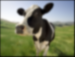
\includegraphics{cow_cubic_smallest}
        (a) 50\%
    \end{minipage}%
    \begin{minipage}{0.35\textwidth}
        \centering
        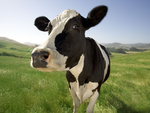
\includegraphics{cow_very_small}
        (b) Original
    \end{minipage}~
    \begin{minipage}{0.35\textwidth}
        \centering
        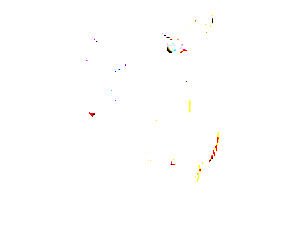
\includegraphics{cow_cubic}
        (c) 150\%
    \end{minipage}
    \caption{Redução e Ampliação com algoritmo de Interpolação Bicúbica}
    \label{fig:vaca:bicubic}
\end{figure}

Na Tabela~\ref{tab:bicubic} vemos os tempos de execução deste algoritmo. Novamente o resultado da redução consta somente como referência, pois a imagem gerada não atende os requisitos do problema.

\begin{table}[H]
    \caption{Tempo de execução}
    \centering
    \label{tab:bicubic}
    \begin{tabular}{c||c}
     Redução & Ampliação \\
     \hline
     0.19s & 0.29s
    \end{tabular}
\end{table}

A Figura~\ref{lst:scale:cubic} mostra o código em Octave para realizar a interpolação bicúbica em uma imagem.

\begin{figure}[H]
\lstinputlisting[language=Octave, lastline=6]{scale-bicubic.m}
\caption{Código-Fonte para interpolação bicúbica no Octave}
\label{lst:scale:cubic}
\end{figure}

Este código é, novamente, muito similar ao da Figura~\ref{lst:scale:linear} e da Figura~\ref{lst:scale:nearest}. A única diferen\c{c}a é na chamada para \textsf{imresize()}, onde se passa o parâmetro \emph{cubic}, que indica que é necessário chamar \textsf{interp2()} com o mesmo parâmetro.

\subsection{Comparação de Resultados}\label{sec:redimensionamento:comparacao}

\section{Rotação}\label{sec:rotacao}

Novamente temos um problema não trivial, com um balanço entre qualidade e eficiência~\cite{kopf:2011}.
\subsection{Rotação por \textit{Nearest Neighbor}}\label{sec:rotacao:nearest}

Podemos ver o resultado na Figura~\ref{fig:vaca:rotacao}.b.

\begin{figure}[H]
\lstinputlisting[language=Octave, lastline=6]{rotate-nearest.m}
\caption{Código-Fonte para rotação por \textit{Nearest Neighbor} no Octave}
\label{lst:rotate:nearest}
\end{figure}

\subsection{Rotação por Interpolação Bilinear}\label{sec:rotacao:bilinear}

\begin{figure}[H]
\lstinputlisting[language=Octave, lastline=6]{rotate-bilinear.m}
\caption{Código-Fonte para rotação por interpolação bilinear no Octave}
\label{lst:rotate:bilinear}
\end{figure}

\subsection{Rotação por Interpolação Bicúbica}\label{sec:rotacao:bicubica}

\begin{figure}[H]
\lstinputlisting[language=Octave, lastline=6]{rotate-bicubic.m}
\caption{Código-Fonte para rotação por interpolação bicúbica no Octave}
\label{lst:rotate:bicubic}
\end{figure}

\subsection{Comparação de Resultados}\label{sec:rotacao:comparacao}

\begin{figure}[H]
    \begin{minipage}{.45\textwidth}
        \centering
        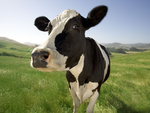
\includegraphics{cow_very_small}
        \\
        (a) Original
    \end{minipage}%
    \begin{minipage}{.45\textwidth}
        \centering
        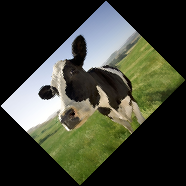
\includegraphics{cow_nearest_rotated}
        (b) \textit{Nearest Neighbor}
    \end{minipage}
    \\
    \begin{minipage}{.45\textwidth}
        \centering
        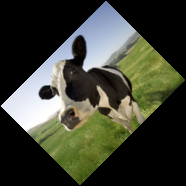
\includegraphics{cow_bilinear_rotated}
        (c) Bilinear
    \end{minipage}%
    \begin{minipage}{.45\textwidth}
        \centering
        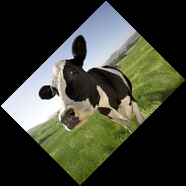
\includegraphics{cow_cubic_rotated}
        (d) Bicúbica
    \end{minipage}
    \caption{Rotação em $45^{\circ}$ por diferentes métodos}
    \label{fig:vaca:rotacao}
\end{figure}

\begin{table}[H]
\centering
\begin{tabular}{c|c|c}
 \textit{Nearest Neighbor} & Bilinear & Bicúbica  \\
 \hline
 0.62 & 0.63 & 2.11
\end{tabular}
\caption{Tempo de execução para rotações (em segundos)}
\label{tab:rotacoes}
\end{table}

\section{Considerações Finais}

\printbibliography

\end{document}
